\chapter{Microphone and Sampling}
%en eller anden indledning til dette afsnit

%det er stadig meget bare hurtige noter, dont judge

\section{Microphone}
In this project an electret microphone is used, since this is the one that is found in telephones. 
Microphones i used to convert sound into a electric signal. This is done by converting oscillations in the air into an oscillating voltage signal. 

\begin{figure}[H]
    \centering
    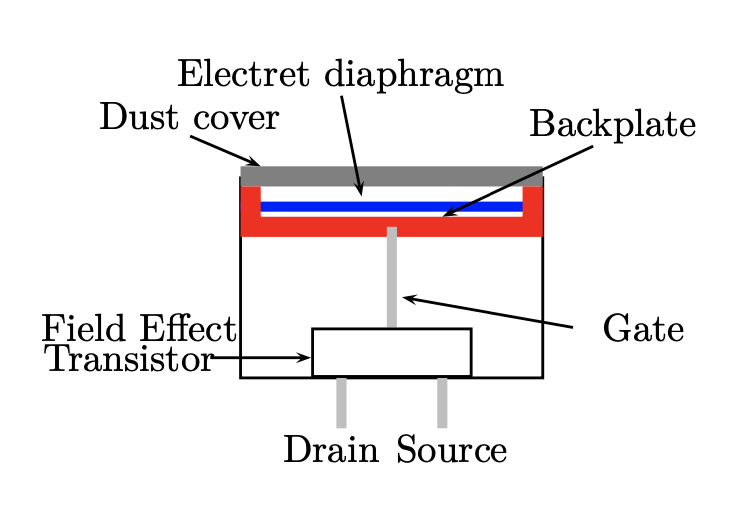
\includegraphics[scale=0.65]{figures/Microphone_figure.png}
    \caption{A figure of an electret microphone \cite[p. 160]{LectureNotes}}
    \label{fig:mic_figure}
\end{figure}

The figure above is a simpler version of a electret microphone. The microphone works by a signal going through the dust cover and then the electret diaphragm will begin to oscillate. When this happens there will be a change in distance between the backplate and the oscillating diaphragm. When this distance changes the capacitance changes and thus will the charge that were on the backplate. There will then be a change in voltage between the diaphragm and the backplate and this is detected by the field effect transistor (FET). The FET can also amplify the voltage. \\

The diaphragm and the backplate creates a capacitor with a capacitance, this can be described by:
$$ C = \dfrac{\varepsilon A}{d}$$ 
where $\varepsilon$ is the permittivity (a measure of the electric polarisation of the electrical insulator), $A$ is the area of the plates and $d$ is the distance between the diaphragm and the backplate. $A$ and $\varepsilon$ is considered constants. $d$ can be described by letting $z(t)$ be the distance between the diaphragm and the backplate to time $t$, by doing this $C$ then becomes a function of $z$. The voltage between the plates and their charge has the relation:
$$
\cite[p. 160]{LectureNotes}

\section{Sampling}
When working with music signal, the music signal is a continuous-time signal.
Going from a continuous-time signal, $x_c(t)$, to a discrete-time signal,$x[n]$, the new discrete-time signal can be manipulated by a computer. A discrete-time signal i essentially a sampled continuous-time signal. The discrete-time signal is formally written as:
$$x={x(n)}, \quad    n \in Z$$
A typical way to obtain a discrete-time signal from a continuous-time signal is by using periodic sampling. A periodic sampling is a sequence of samples, $x[n]$, also referred to as the nth sample, obtained from the continuous-time signal,$x_c(t)$, by using the following relation:
$$x[n]=xc (nT), \quad    - \infty <n< \infty$$

where $T$ is the sampling period and it is from the relation $f=\dfrac{1}{T}$, where $f$ is the sampling frequency, in samples per second. This can also be called a C/D converter, ideal continuous to discrete converter. 
By using a A/D converter, analog to digital converter, an approximation of the C/D conversion is achieved. \cite[p. 140-142]{DiscreteTimeSignal}
